\documentclass[journal]{IEEEtran}
\usepackage[a5paper, margin=10mm, onecolumn]{geometry}
\usepackage{lmodern}
\usepackage{tfrupee}
\setlength{\headheight}{1cm}
\setlength{\headsep}{0mm}

\usepackage{gvv-book}
\usepackage{gvv}
\usepackage{cite}
\usepackage{amsmath,amssymb,amsfonts,amsthm}
\usepackage{algorithmic}
\usepackage{graphicx}
\usepackage{textcomp}
\usepackage{xcolor}
\usepackage{txfonts}
\usepackage{listings}
\usepackage{enumitem}
\usepackage{mathtools}
\usepackage{gensymb}
\usepackage{comment}
\usepackage[breaklinks=true]{hyperref}
\usepackage{tkz-euclide}
\usepackage{listings}
\def\inputGnumericTable{}
\usepackage[latin1]{inputenc}
\usepackage{color}
\usepackage{array}
\usepackage{longtable}
\usepackage{calc}
\usepackage{multirow}
\usepackage{hhline}
\usepackage{ifthen}
\usepackage{lscape}
\usepackage{xparse}

\bibliographystyle{IEEEtran}

\title{5.8.40}
\author{EE25BTECH11043 - Nishid Khandagre} 

\begin{document}
\maketitle

\renewcommand{\thefigure}{\theenumi}
\renewcommand{\thetable}{\theenumi}

\numberwithin{equation}{enumi}
\numberwithin{figure}{enumi}

\textbf{Question}:\
The ratio of incomes of two persons is 9:7 and the ratio of their expenditures is 4:3. If each of them manages to save rupees 2000 per month, find their monthly incomes.

\textbf{Solution: }
Let the monthly incomes be $x$ and $y$.

Given income ratio:
    \begin{align}
    \frac{x}{y} &= \frac{9}{7} \\
    7x - 9y &= 0
    \end{align}
Expenditures are Income $-$ Savings.
Expenditures are $x-2000$ and $y-2000$.
Given expenditure ratio:
    \begin{align}
    \frac{x-2000}{y-2000} &= \frac{4}{3} \\
    3x - 6000 &= 4y - 8000 \\
    3x - 4y &= -2000
    \end{align}

    \begin{align}
    7x - 9y &= 0 \\
    3x - 4y &= -2000
    \end{align}
    Matrix form:
    \begin{align}
    \myvec{7 & -9 \\ 3 & -4}
    \myvec{x \\ y}
    =
    \myvec{0 \\ -2000}
    \end{align}
    Augmented matrix:
    \begin{align}
    \myaugvec{2}
    {
    7 & -9 & 0 \\
    3 & -4 & -2000 \\
    }
    \end{align}

 
    
    Then $R_2 \rightarrow 7R_2 - 3R_1$
    \begin{align}
    \myaugvec{2}{
    7 & -9 & 0 \\
    0 & -1 & -14000
    }
    \end{align}


    Then $R_2 \rightarrow -R_2$
    \begin{align}
    \myaugvec{2}{
     7 & -9 & 0 \\
     0 & 1 & 14000
    }
    \end{align}

    Then $R_1 \rightarrow R_1 + 9R_2$ 
    \begin{align}
    \myaugvec{2}{
    7 & 0 & 126000 \\
    0 & 1 & 14000
    }
    \end{align}

    Then $R_1 \rightarrow \frac{1}{7}R_1$
    
    \begin{align}
        \myaugvec{2}{
        1 & 0 & 18000 \\
        0 & 1 & 14000
       }
        \end{align}
   
    \begin{align}
    \myvec{x\\y}&=\myvec{18000\\14000}
    \end{align}
    
    \begin{align}
    x &= 18000 \\
    y &= 14000
    \end{align}
    Thus, the monthly incomes are \rupee{18000} and \rupee{14000}.

\begin{figure}[H]
    \centering
    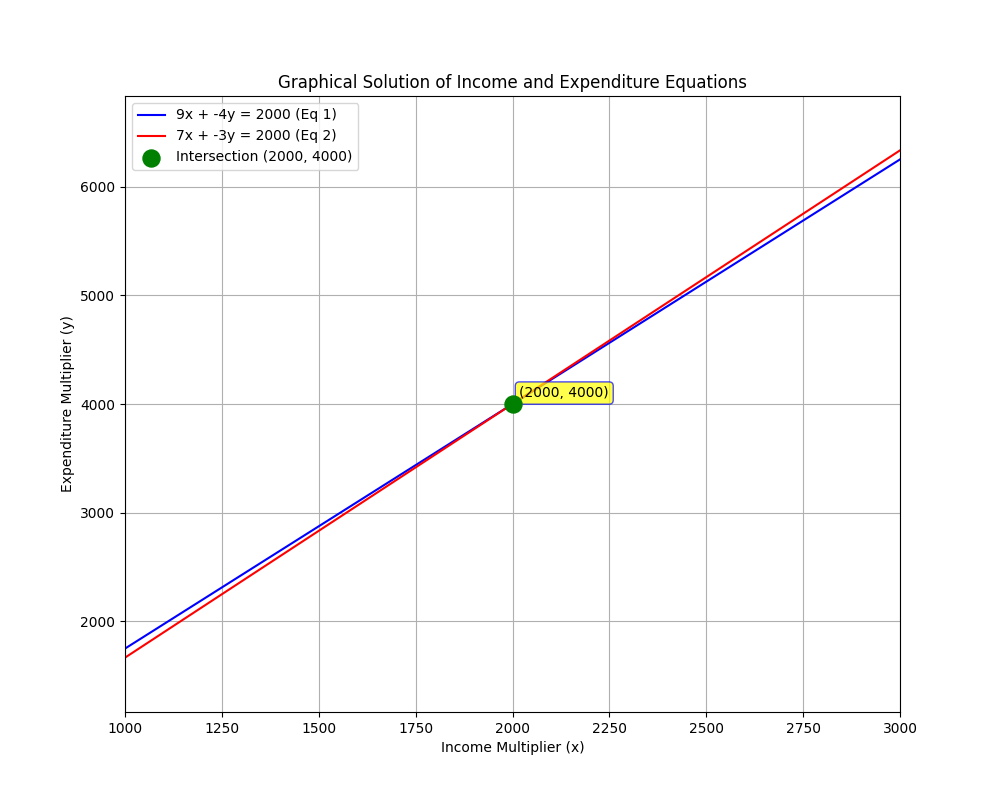
\includegraphics[width=0.8\columnwidth]{figs/fig1.png}
    \caption{}
    \label{fig:1}
\end{figure}



\end{document}
